\section{Security Analysis}
\label{sec:security}

The rest of this section describes the security properties of
enclaves, discussing the trade-offs made while trying to balance security with
backwards compatibility.



% ECREATE forces R, W, X to 0 in the page's EPCM. EADD also forces R/W/X to 0
% if the page type in SECINFO is PT_TCS (the only special type it can create).
%
%
% EPA doesn't read any SECINFO, and uses 0 for R, W, X.

% ERESUME can be replaced by normal EENTER, XRESTOR and accounting. Describe
% and argue against ERESUME.


% The use of the page version (nonce) as counter in AES-GCM makes it impossible
% for malicious system software to determine whether an EPC page's contents has
% changed between two evictions.
% However, the dirty bit in the EPC page's PTE will leak that information.

% According to the ECREATE pseudo-code in the Intel manual, EIDs are assigned
% using a counter that is atomically incremented on every ECREATE. This makes
% the field predictible to system software.


% The SGX instruction that evicts an EPC page, EWB, ensures that the VA slot it
% is supposed to write is unused.
% The VA unused slot check in EWB is unnecessary. Bad system software can only
% overwrite a version and impair its ability to restore a page.

Enclaves were designed to contain and protect the privacy-sensitive parts of an
application. All the code that handles private data must receive integrity
protection. Otherwise, a hostile environment could modify the code to leak
information about private data. Therefore, the SGX programming model prescribes
that code which accesses private data must be entirely contained inside an
enclave. Jumping into and out of enclave code must be performed explicitly
using the dedicated instructions \texttt{EENTER} and \texttt{EEXIT}.


% Victor 2 scheme for ETRACK / EBLOCK / EWB.
%
% ETRACK - sets tracking to 1, sets CPUmask in SECS to 0, sets LPleft to number
%          of logical processors executing enclave code, sets canEvict to 0
% EEXIT / AEX - if tracking is set to 1 and CPUmask bit in SECS for current LP
%               is set to 0, decrement LPleft; if LPleft is 0, set canEvict to
%               1
% EENTER - if tracking is set to 1, set CPUmask bit in SECS for current LP to 1
% EWB - check that canEvict is 1; set tracking to 0


\begin{figure}[hbt]
  \centering
  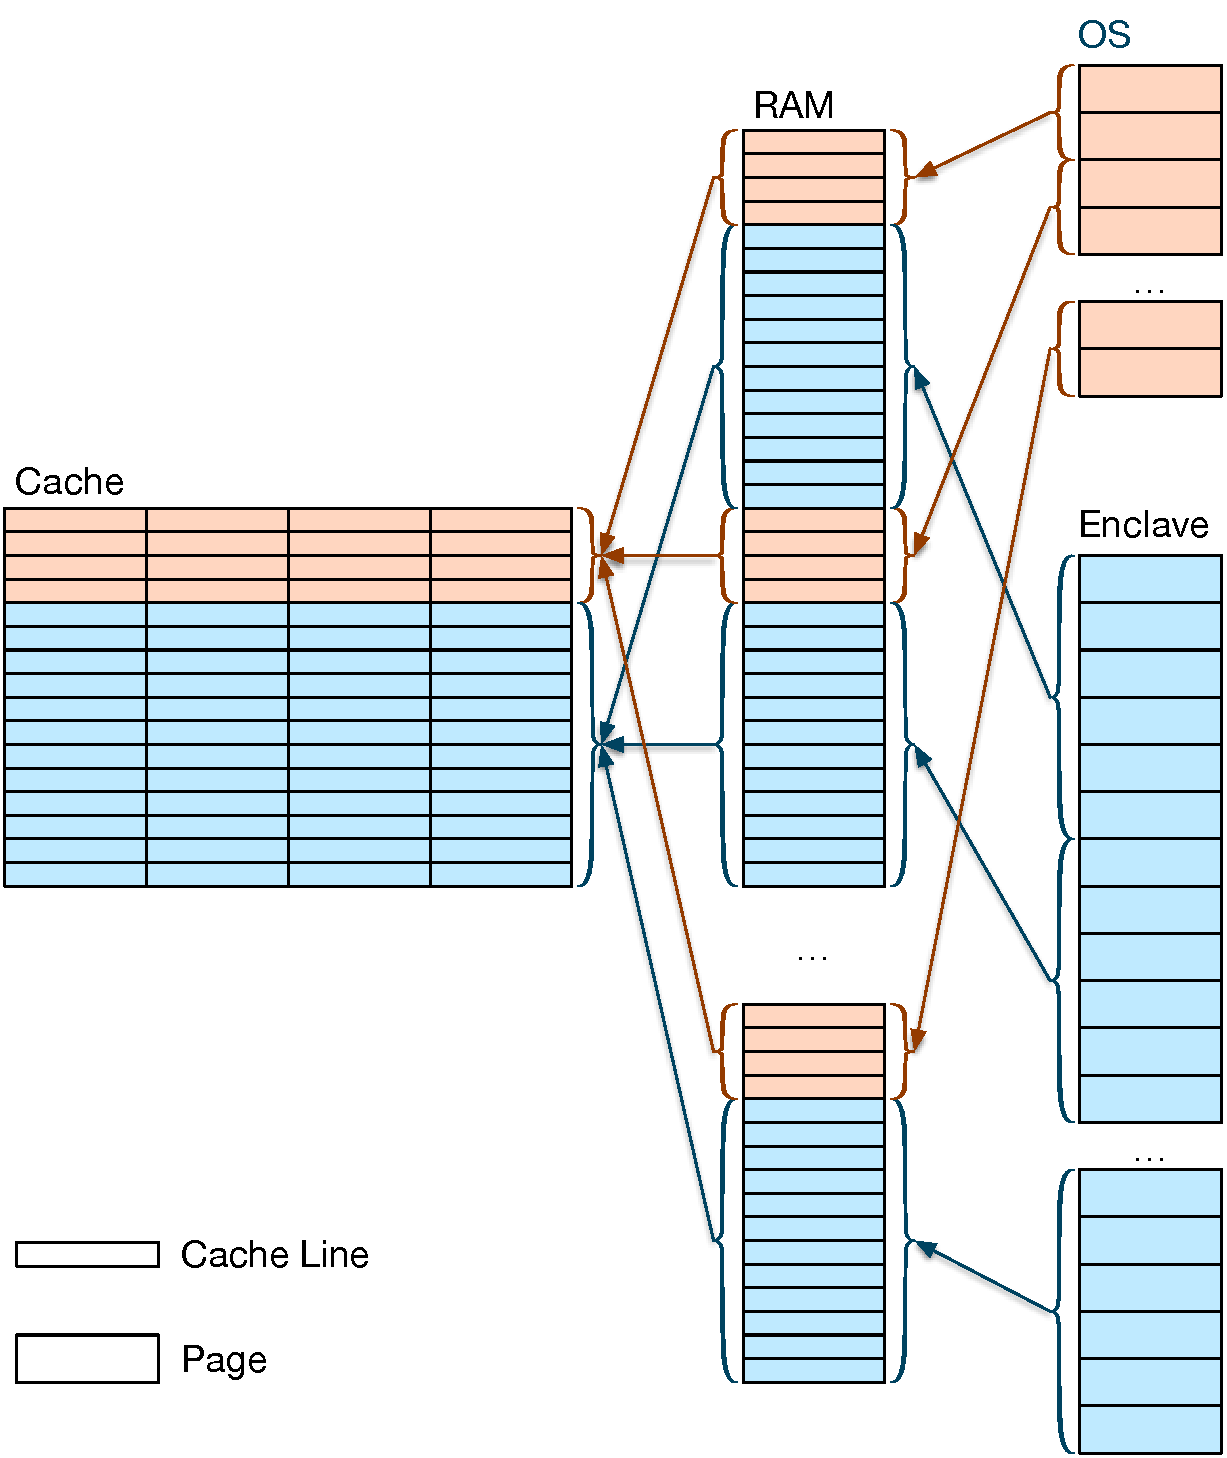
\includegraphics[width=85mm]{figures/cache_partitions.pdf}
  \caption{
    Cache partitioning between two applications. Each application has some
    cache sets allocated to it, and only uses RAM regions that map to its cache
    sets. When partitioning the L1 cache, applications have to follow this
    constraint themselves. When the L2 cache is partitioned, the OS can map the
    pages in an application's virtual address space to the RAM regions that the
    application can use, so applications are oblivious to the cache
    partitioning.
  }
  \label{fig:cache_partitions}
\end{figure}


\subsection {Page Eviction Security}

The most obvious attack is prevented by having the MAC cover the contents of
the evicted EPC page, so the untrusted OS cannot modify the data in the page
while it is stored in untrusted DRAM. The MAC also covers the metadata that
makes up the EPCM entry, which prevents the more subtle attacks described
below.

The enclave ID (EID) field is covered by the MAC tag, so the OS cannot evict an
EPC page belonging to one enclave, and assign the page to a different enclave
when it is loaded back into the EPC. If EID was not covered by authenticity
guarantees, a malicious OS could read any enclave's data by evicting an EPC
page belonging to the victim enclave, and loading it into a malicious enclave
that would copy the page's contents to untrusted DRAM.

The virtual address (LINADDR) field is covered by the MAC tag, so the OS cannot
modify the virtual memory layout of an enclave by evicting an EPC page and
specifying a different LINADDR when loading it back. If LINADDR was not covered
by authenticity guarantees, a malicious OS could perform the exact attack shown
in Figure~\ref{fig:swap_mapping_attack} and described in
\S~\ref{sec:page_swapping_attacks}.

The page access permission flags (R, W, X) are also covered by the MAC tag.
This prevents the OS from changing the access permission bits in a page's EPCM
entry by evicting the page and loading it back in. If the permission flags were
not covered by authenticity guarantees, the OS could use the ability to change
EPCM access permissions to facilitate exploiting vulnerabilities in enclave
code. For example, exploiting a stack overflow vulnerability is generally
easier if OS can make the stack pages executable.

The nonce stored in the VA slot is also covered by the MAC. This prevents the
OS from mounting a replay attack that reverts the contents of an EPC page to an
older version. If the nonce would not be covered by integrity guarantees, the
OS could evict the target EPC page at different times $t_1$ and $t_2$ in the
enclave's life, and then provide the \texttt{EWB} outputs at $t_1$ to the
\texttt{ELDU} / \texttt{ELDB} instruction. Without the MAC verification, this
attack would successfully revert the contents of the EPC page to its version
at $t_1$.

While replay attacks look relatively benign, they can be quite devastating when
used to facilitate double spending.


\subsubsection{On Measuring Enclave Attributes}

At a very high level, the exponential explosion described here seems similar to
the measurement problem that plauges the Trusted Platform
Module~(TPM,~\S~\ref{sec:tpm}). However, they are quite different. The TPM's
measurement must account for all the system \textbf{software} loaded on the
computer, including all the drivers. The explosion of potentially valid TPM
measurement is due to the fact that every new OS kernel release and driver
release creates new potentially valid measurements. If SGX were to include XFRM
values into the enclave's measurement, the number of possible \textbf{hardware}



\subsection{DOS Prevention}
% NOTE: This is a slightly edited answer to a question we received.

SGX enclaves execute at the lowest privilege level (user mode / ring 3), so
they cannot compromise the system software without exploiting a security
vulnerability. Therefore, the only kind of malicious behavior that an enclave
can exhibit is denial of service (DoS).

The SGX design provides system software the tools it needs to protect itself
from enclaves that engage into CPU hogging and DRAM hogging. As enclaves cannot
perform I/O directly, these are the only two classes of DoS attacks available
to them.

An enclave that attempts to hog a logical processor (CPU core on most systems)
assigned to it can be pre-empted by the system software via an Inter-Processor
Interrupt (IPI) issued from another processor. This method is available as long
as the system software reserves at least one logical processor for non-enclave
computation.

Furthermore, most OS kernels use tick schedulers, which use a real-time clock
(RTC) configured to issue periodical interrupts (ticks) to all cores. The RTC
interrupt handler invokes the kernel's scheduler, which choses the thread that
will get to use the logical processor until the next RTC interrupt is received.
Therefore, kernels that use tick schedulers always have the opportunity to
de-schedule enclave threads, and don't need to rely on the ability to send
IPIs.

In SGX, the system software can always evict an enclave's EPC pages to non-EPC
memory, and then to disk. The system software can also outright deallocate an
enclave's EPC pages, though this will probably cause the enclave code to
encounter page faults that cannot be resolved. The only catch is that the EPC
pages that hold metadata for running enclave threads cannot be evicted or
removed. However, this can easily be resolved, as the system software can
always preempt enclave threads, using one of the methods described above.

% TODO(pwnall): Move the following paragraphs into Sanctum.

Sanctum gives the system software less control over the DRAM regions allocated
to enclaves, in order to hide the enclaves' memory access patterns.
Specifically, the system software cannot reclaim a DRAM region from an enclave
without the enclave's cooperation. However, the system software can always
completely terminate an enclave and reclaim all its memory.

Sanctum's enclaves can only be terminated when all their threads are stopped.
Therefore, when the system software decides that an enclave is hogging CPU or
DRAM, it can pre-empt all the enclave's threads, using the methods described
above, and then terminate the enclave.


\subsection{Interaction with Anti-Virus Software}
% NOTE: This is a slightly edited answer to a question we received.

Today's anti-virus (AV) systems are glorified pattern matchers. AV software
simply scans all the executable files on the system and the memory of running
processes, looking for bit patterns that are thought to only occur in malicious
software. These patterns are pompously called "virus signatures".

SGX (and TXT, to some extent) provides a method for executing code in an
isolated container that we refer to as an enclave. Enclaves are isolated from
all the other software on the computer, including any AV software that might be
installed.

The isolation afforded by Sanctum (and SGX, etc.) opens up the possibility for
bad actors to structure their attacks as a generic loader that would end up
executing a malicious payload without tripping the AV's pattern matcher.  More
specifically, the attack would create an enclave and initialize it with a
generic loader that looks innocent to an AV. The loader inside the enclave
would obtain an encrypted malicious payload, and would undergo software
attestation with an Internet server to obtain the payload's encryption key. The
loader would then decrypt the malicious payload and execute it inside the
enclave.

In the scheme suggested here, the malicious payload only exists in a decrypted
form inside an enclave's memory, which cannot be accessed by the AV. Therefore,
the AV's pattern matcher will not trip.

This issue does not have a solution that maintains the status-quo for the AV
vendors. The attack described above would be called a protection scheme if the
payload would be a proprietary image processing algorithm, or a DRM scheme.

On a brighter note, enclaves do not bring the complete extinction of AV, they
merely require a change in approach. Enclave code always executes at the lowest
privilege mode (ring 3 / user mode), so it cannot perform any I/O without
invoking the services of system software. For all intents and purposes, this
effectively means that enclave software cannot perform any malicious action
without the complicity of system software. Therefore, enclaves can be policed
effectively by intelligent AV software that records and filters the I/O
performed by software, and detects malicious software according to the actions
that it performs, rather than according to bit patterns in its code.

Furthermore, SGX's enclave loading model allows the possibility of performing
static analysis on the enclave's software. For simplicity, assume the existence
of a standardized static analysis framework.  The initial enclave contents is
not encrypted, so the system software can easily perform static analysis on it.
Dynamically loaded code or Just-In-Time code generation (JIT) can be handled by
requiring that all enclaves that use these techniques embed the static analysis
framework and use it to analyze any dynamically loaded code before it is
executed. The system software can use static verification to ensure that
enclaves follow these rules, and refuse to initialize any enclaves that fail
verification.

In conclusion, enclaves in and of themselves don't introduce new attack vectors
for malware. However, the enclave isolation mechanism is fundamentally
incompatible with the approach employed by today's AV solutions. Fortunately,
it is possible (though non-trivial) to develop more intelligent AV software for
enclave software.


\subsection{SGX Information Leaks}
\label{sec:sgx_leaks}

Software Guard Extensions, as documented in \cite{intel2015sdm}, does not
provide full privacy guarantees to the code executing inside an enclave. We
present methods that an attacker can use to extract information from an
enclave.

\subsubsection{Hyper-Threading Leaks}

Modern Intel CPUs feature hyper-threading, which means that each core has two
(or more) sets of register files and local APICs, presented as logical
processors running separate threads (see Figure \ref{fig:cpu_core}). The
threads share the other core resources, such as the fetch and decode units,
execution units and L1 and L2 caches. SGX does not prevent hyper-threading, so
a malicious OS kernel or hypervisor can schedule a thread executing enclave
code and a snooping thread on logical processors on same core. The snooping
thread can use the processor's high-resolution performance counter
\cite{petters1999making} to get information about the instructions and memory
access patterns of the thread executing enclave code.

A promising approach for preventing against hyper-threading leaks is to
effectively disable hyper-threading, by using \texttt{CPUID} to find out the
number of logical processors in the current core, and to require the OS to
schedule threads in the same enclave on all the logical processors. This could
be implemented by having the main thread spinlock waiting for the other threads
to start, before any protected computation is performed. However, a malicious
kernel or hypervisor can de-schedule the other threads after the main thread
performed the spinlock check, so this defense is not reliable.

\subsubsection{Page-Level Memory Access Leaks}

While executing the code inside an enclave, the CPU still follows the standard
page translation process (\S \ref{sec:paging}), including setting the A and D
bits and delivering page faults. A malicious OS kernel or hypervisor can
obtain the page-level trace of an application executing inside an enclave by
setting the P flag to 0 on all the enclave's pages before starting enclave
execution, and then maintaining exactly one instruction page and one data page
present in the enclave's address space.

When a page fault is generated, CR2 contains the virtual address of a page
accessed by enclave, and the error code indicates whether the memory access was
a read or a write (bit 1) and whether the memory access is a data access or
an instruction fetch access (bit 4). On a data access, the kernel tracing the
enclave code's memory access pattern would set the P flag of the desired page
to 1, and set the P flag of the previously accessed data page to 0. Instruction
accesses can be handled in a similar manner.

For a slightly more detailed trace, the kernel can set a desired page's W flag
to 0 if the page fault's error code indicates a read access, and only set it to
1 for write accesses. Also, applications that use a page as both code and data
(self-modifying code and just-in-time compiling VMs) can be handled by setting
a page's XD flag to 0 for a data access, and by carefully accounting for the
case where the last accessed data page is the same as the last accessed code
page.

Leaving an enclave via an AEX and re-entering the enclave via \texttt{ERESUME}
causes the CPU to flush TLB entries that contain enclave addresses, so a
tracing kernel would not need to worry about flushing the TLB. The tracing
kernel does not need to flush the caches either, because the CPU needs to
perform address translation even for cached data.

An easy way to reduce this attack's power is to increase the page size, so the
trace contains less information. However, the attack cannot be completely
prevented without removing the kernel's ability to oversubscribe the EPC,
which is a major benefit of paging.

\subsubsection{Fine-Grained Memory Access Leaks}

The AEX process and the \texttt{ERESUME} instructions do not flush the CPU
caches. A tracing kernel can take advantage of cache timing to narrow down
the addresses in an application's memory access trace to cache line
granularity, by extending the method described above with the steps below.

The tracing kernel controls the mapping between virtual addresses and physical
addresses, so it can make sure that its own code and data use different sets
in the L2 cache from the enclave's code and data. For example, in a typical
256~KB (per-core) L2 cache organized as 512 8-way sets of 64-byte lines, the
tracing kernel could allocate lines 0-63 for the enclave's code page, lines
64-127 for the enclave's data page, and use lines 128-511 for its own pages.

Right before entering an enclave via \texttt{EENTER} or \texttt{ERESUME}, the
kernel would issue \texttt{CLFLUSH} instructions to flush the enclave's code
page and data page from the cache. The enclave could have accessed a single
code page and a single data page, so flushing the cache should be reasonably
efficient. The tracing kernel then uses 16 bogus pages (8 for the enclave's
code page, and 8 for the enclave's data page) to load all the 8 ways in the 128
cache sets allocated by enclave pages. After an AEX gives control back to the
tracing kernel, it can read the 16 bogus pages, and exploit the time difference
between an L2 cache hit and a miss to see which cache lines were evicted and
replaced by the enclave's memory accesses.

\subsubsection{Leaks via Physical Attacks}

The methods described above rely on a compromised hypervisor or OS kernel, but
not on physical attacks. If an attacker can tap into the memory bus and read
the address lines, the attacker can learn the enclave code's memory access
patterns, at a fine granularity.

The processor reserved memory (PRM) is configured by the BIOS at boot time as
a continuous memory area, and can be configured as write-back (WB) or
uncacheable (UC) memory. If the PRM is uncacheable, the CPU will generate a
memory transaction for every memory access. The granularity of the memory
transactions depends on the encryption engine used for the EPC, which is not
documented in \cite{intel2015sdm}. If 128-bit AES is used, memory tapping
would yield addresses at 16-byte granularity, which means two 64-bit words.

At the same time, configuring the PRM as uncacheable memory removes the cache
timing attack documented above, at the cost of dramatically slowing down the
execution of SGX code. In this case, the CPU would still leak memory access
patterns at page granularity, due to the address translation engine.
